% METTI SOLO TABELLE E GRAFICI, SU RETROSPETTIVA FAI UNA TABELLA RIASSUNTIVA E COMMENTA I PROBLEMI
\paragraph{MS001 - Numero di metodi}\mbox{}\\[0,3cm]
    \begin{table}[H]
        \centering
        \begin{tabular}{ccccccc}
            \rowcolor{greySWEight}
            \textcolor{white}{\textbf{Codice}} &
            \textcolor{white}{\textbf{File analizzati}}&
            \textcolor{white}{\textbf{Media metodi per classe}}&
            \textcolor{white}{\textbf{Riscontro}}\\
            \textbf{MS001} & 79 & 2.46 & \textcolor{ForestGreen}{Ottimale}\\
        \end{tabular}
        \caption{Media metodi per classe}
    \end{table}

    \begin{figure}[H]
        \centering
        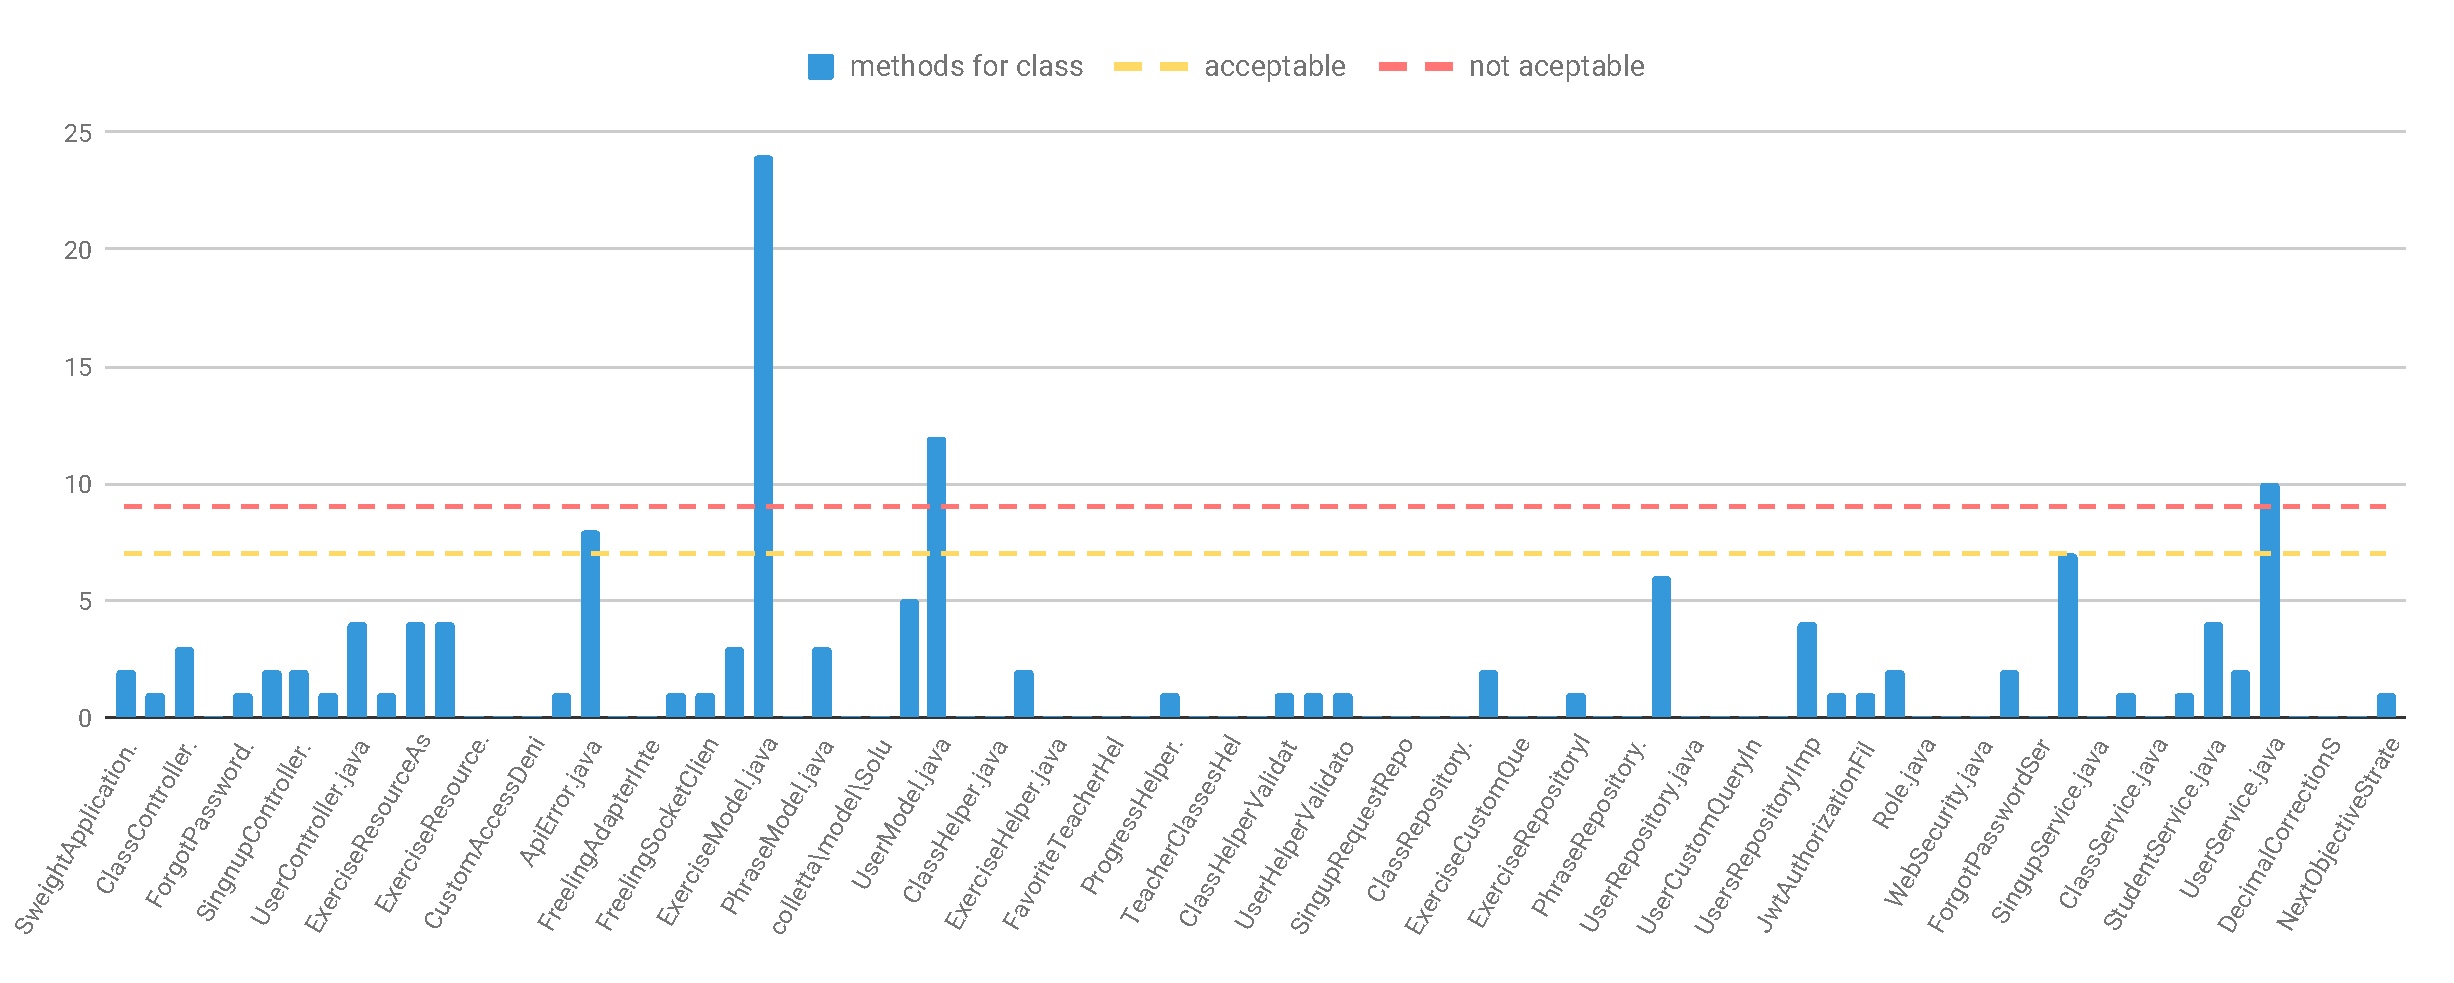
\includegraphics[width=165mm]{sez/App_Esito/Approvazione/graph/metodi.pdf}
        \caption{Metodi per classe alla revisione di Approvazione}
    \end{figure}

    \begin{figure}[H]
        \centering
        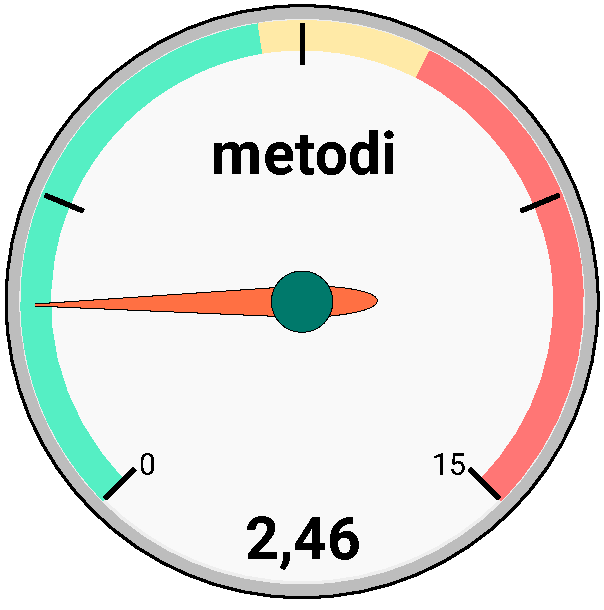
\includegraphics[width=45mm]{sez/App_Esito/Approvazione/graph/metodiCruscotto.pdf}
        \caption{Media metodi per classe alla revisione di Approvazione}
    \end{figure}

\paragraph{MS002 - Numero di parametri}\mbox{}\\[0,3cm]
    \begin{table}[H]
        \centering
        \begin{tabular}{cccccc}
            \rowcolor{greySWEight}
            \textcolor{white}{\textbf{Codice}} &
            \textcolor{white}{\textbf{Files}} &
            \textcolor{white}{\textbf{Metodi}}&
            \textcolor{white}{\textbf{Accettabile}}&
            \textcolor{white}{\textbf{Non accettabile}}&
            \textcolor{white}{\textbf{Riscontro}}\\
            \textbf{MS001} & 79 & 134 & 1 & 0 &\textcolor{YellowOrange}{Accettabile}\\
        \end{tabular}
        \caption{Parametri dei metodi alla revisione di Approvazione}
    \end{table}

    \begin{figure}[H]
        \centering
        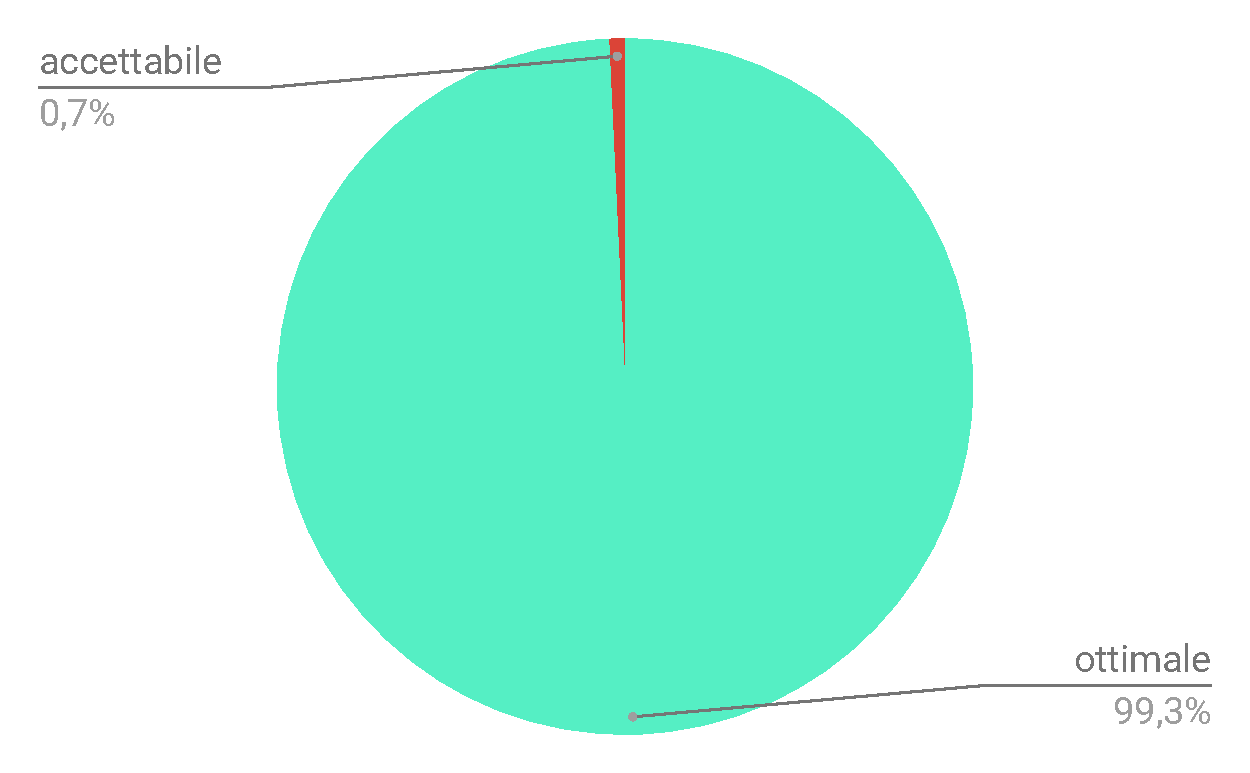
\includegraphics[width=100mm]{sez/App_Esito/Approvazione/graph/parametri.pdf}
        \caption{Percentuale valori dei parametri superati alla revisione di approvazione}
    \end{figure}

\paragraph{MS003 - Funzioni di interfaccia per package}\mbox{}\\[0,3cm]
    \begin{table}[H]
        \centering
        \begin{tabular}{ccccc}
            \rowcolor{greySWEight}
            \textcolor{white}{\textbf{Codice}} &
            \textcolor{white}{\textbf{File analizzati}} &
            \textcolor{white}{\textbf{Media}}&
            \textcolor{white}{\textbf{Riscontro}}\\
            \textbf{MS003} & 79 & 0.61 & \textcolor{ForestGreen}{Ottimale}\\
        \end{tabular}
        \caption{Numero interfacce per package}
    \end{table}
    \begin{figure}[H]
        \centering
        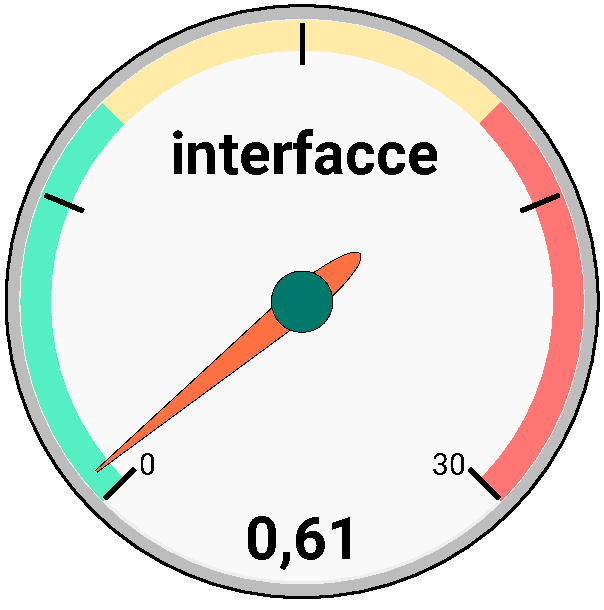
\includegraphics[width=45mm]{sez/App_Esito/Approvazione/graph/interfacceCruscotto.pdf}
        \caption{Interfacce per package alla revisione di Approvazione}
    \end{figure}
    \begin{figure}[H]
        \centering
        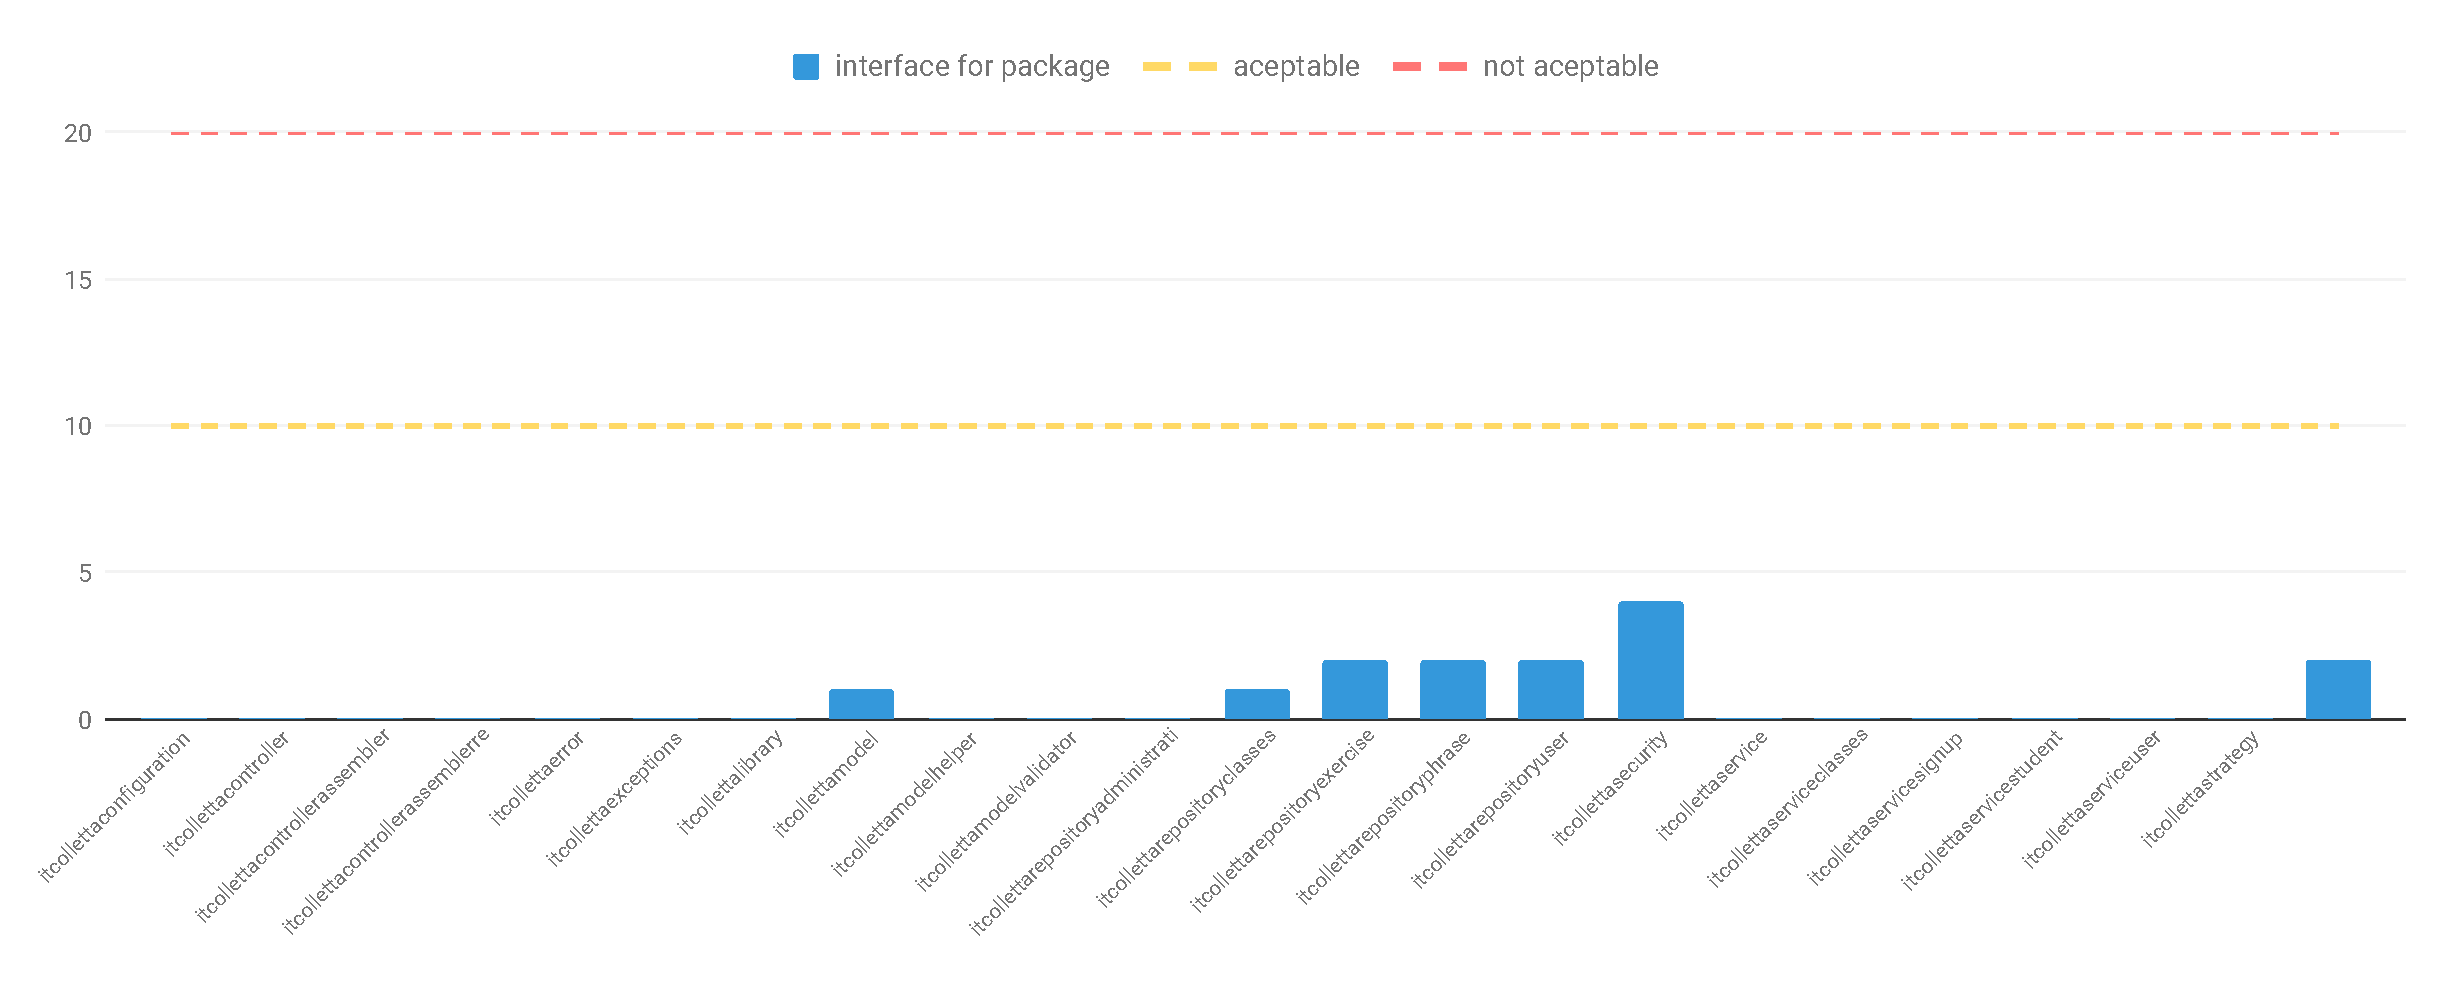
\includegraphics[width=165mm]{sez/App_Esito/Approvazione/graph/interfacce.pdf}
        \caption{Interfacce per package alla revisione di Approvazione}
    \end{figure}

\paragraph{MS004 - Complessità ciclomatica}\mbox{}\\[0,3cm]
    \begin{table}[H]
        \centering
        \begin{tabular}{ccccccc}
            \rowcolor{greySWEight}
            \textcolor{white}{\textbf{Codice}} &
            \textcolor{white}{\textbf{File analizzati}} &
            \textcolor{white}{\textbf{Valore}}&
            \textcolor{white}{\textbf{Riscontro}}\\
            \textbf{MS004} & 79 & 1.35 & \textcolor{ForestGreen}{Ottimale}\\
        \end{tabular}
        \caption{Complessità ciclomatica alla revisione di Approvazione}
    \end{table}
    \begin{figure}[H]
        \centering
        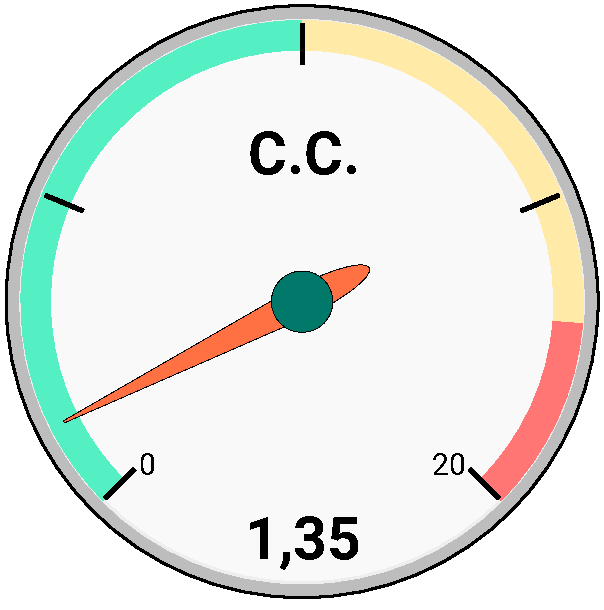
\includegraphics[width=45mm]{sez/App_Esito/Approvazione/graph/complessitaCiclomatica.pdf}
        \caption{Cruscotto complessità ciclomatica alla revisione di Approvazione}
    \end{figure}

\paragraph{MS005 - Campi dati per classe}\mbox{}\\[0,3cm]
    \begin{table}[H]
        \centering
        \begin{tabular}{ccccccc}
            \rowcolor{greySWEight}
            \textcolor{white}{\textbf{Codice}} &
            \textcolor{white}{\textbf{File analizzati}}&
            \textcolor{white}{\textbf{[10,15] campi dati}}&
            \textcolor{white}{\textbf{15 o più campi dati}}&
            \textcolor{white}{\textbf{Riscontro}}\\
            \textbf{MS005} & 79 & 3 & 0 & \textcolor{YellowOrange}{Accettabile}\\
        \end{tabular}
        \caption{Campi dati per classe alla revisione di Approvazione}
    \end{table}
    \begin{figure}[H]
        \centering
        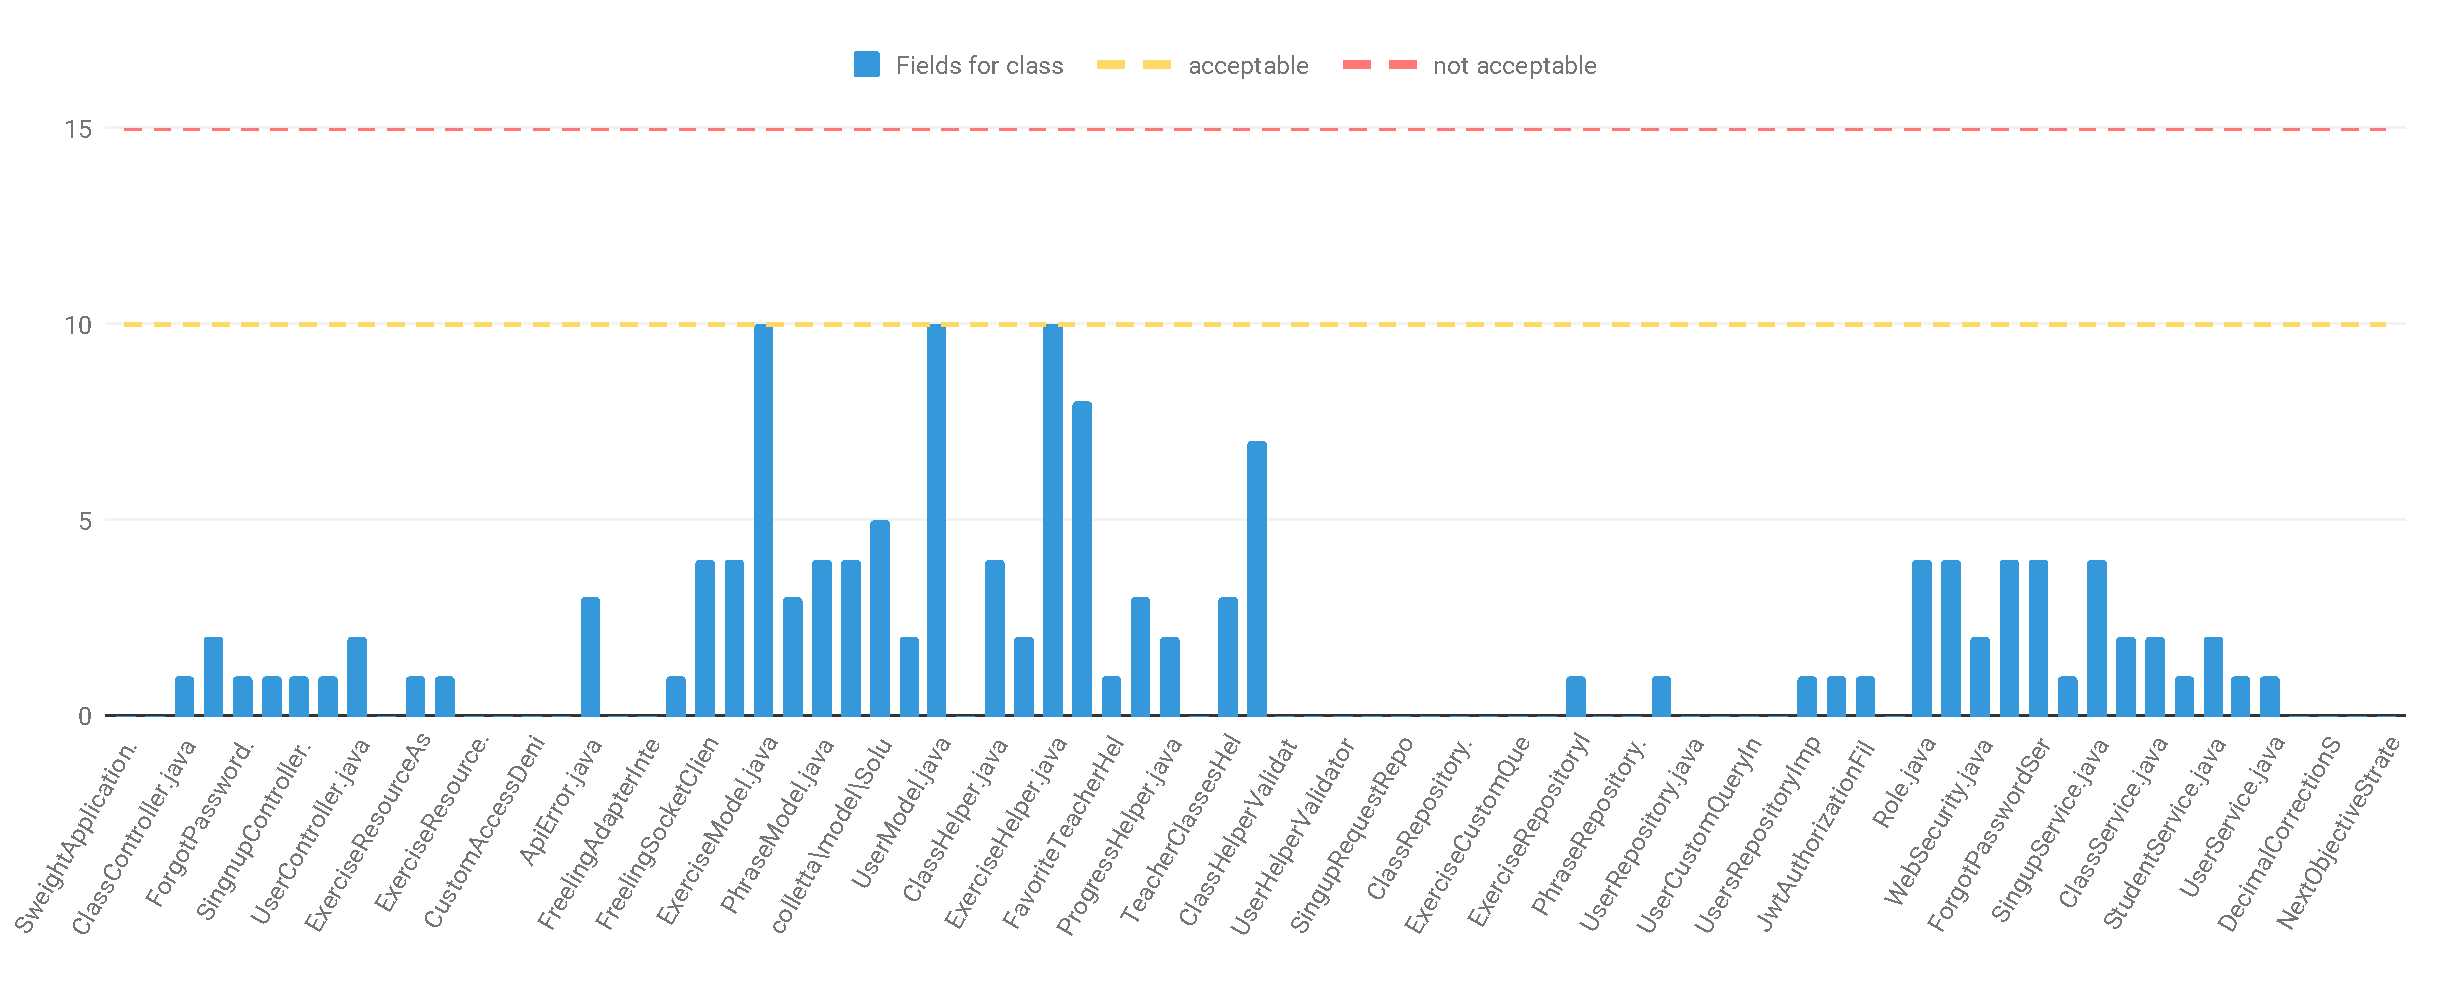
\includegraphics[width=165mm]{sez/App_Esito/Approvazione/graph/campiDati.pdf}
        \caption{Numero di campi dati per classe alla revisione di Approvazione}
    \end{figure}
    \begin{figure}[H]
        \centering
        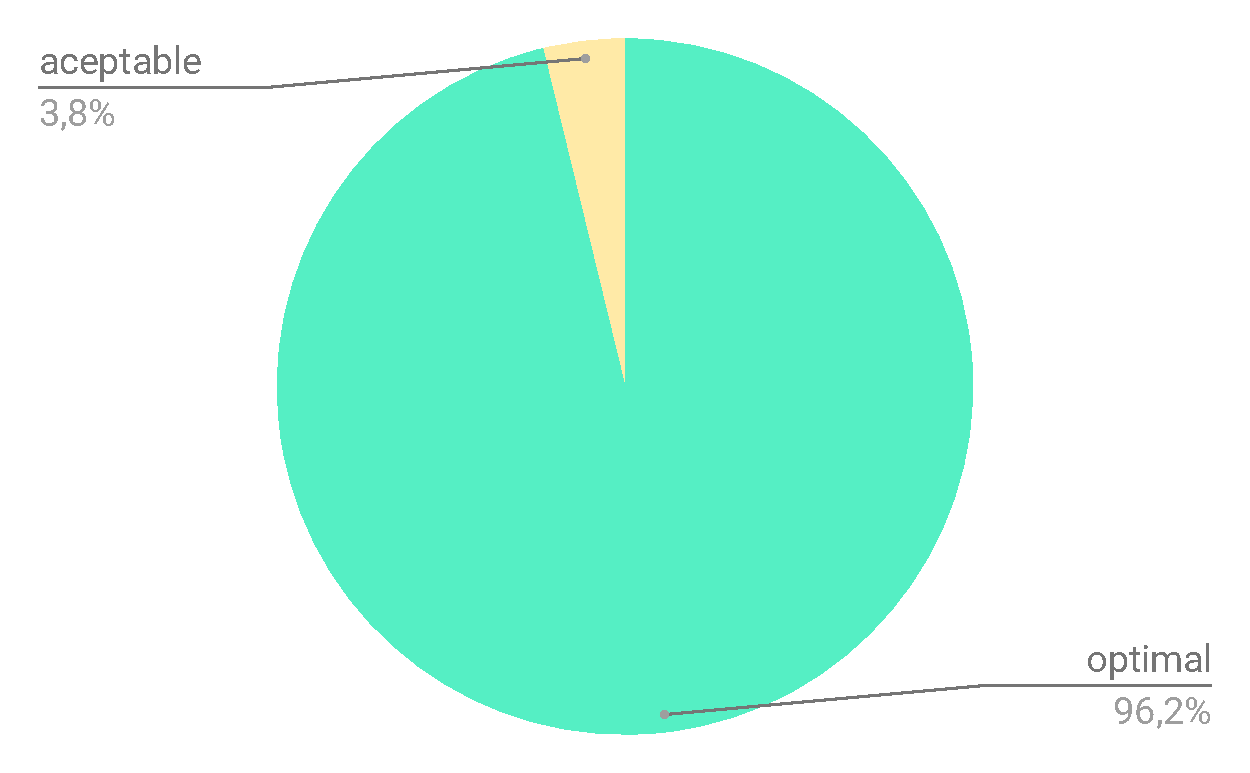
\includegraphics[width=100mm]{sez/App_Esito/Approvazione/graph/campiDatoTorta.pdf}
        \caption{Percentuale valore dei campi dati superati alla revisione di Approvazione}
    \end{figure}

\paragraph{MS006 - Commenti per linee di codice}\mbox{}\\[0,3cm]
    \begin{table}[H]
        \centering
        \begin{tabular}{ccccccc}
            \rowcolor{greySWEight}
            \textcolor{white}{\textbf{Codice}} &
            \textcolor{white}{\textbf{File analizzati}}&
            \textcolor{white}{\textbf{Totale righe}}&
            \textcolor{white}{\textbf{Totale righe commento}}&
            \textcolor{white}{\textbf{Percentuale}}&
            \textcolor{white}{\textbf{Riscontro}}\\
            \textbf{MS006} & 153 & 14001 & 1533 & 11.34\% & \textcolor{YellowOrange}{Accettabile}\\
        \end{tabular}
        \caption{Totale commenti per linee di codice nel periodo di Codifica}
    \end{table}
    \begin{figure}[H]
        \centering
        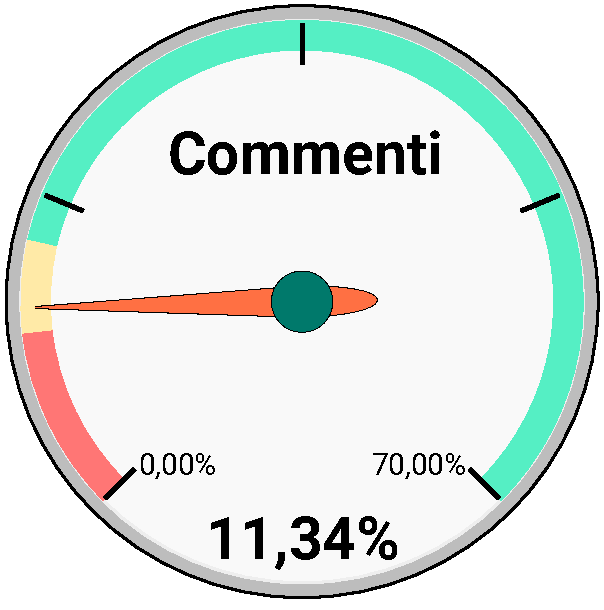
\includegraphics[width=45mm]{sez/App_Esito/Approvazione/graph/commenti.pdf}
        \caption{Commenti per linee di codice alla revisione di Approvazione}
    \end{figure}
    

\paragraph{MS007 - Code coverage}\mbox{}\\[0,3cm]
    \begin{table}[H]
        \centering
        \begin{tabular}{ccccc}
            \rowcolor{greySWEight}
            \textcolor{white}{\textbf{Codice}} &
            \textcolor{white}{\textbf{Valore}}&
            \textcolor{white}{\textbf{Riscontro}}\\
            \textbf{MS007} & 83.1\% & \textcolor{YellowOrange}{Accettabile}\\
        \end{tabular}
        \caption{Code coverage alla revisione di Approvazione}
    \end{table}
    \begin{figure}[H]
        \centering
        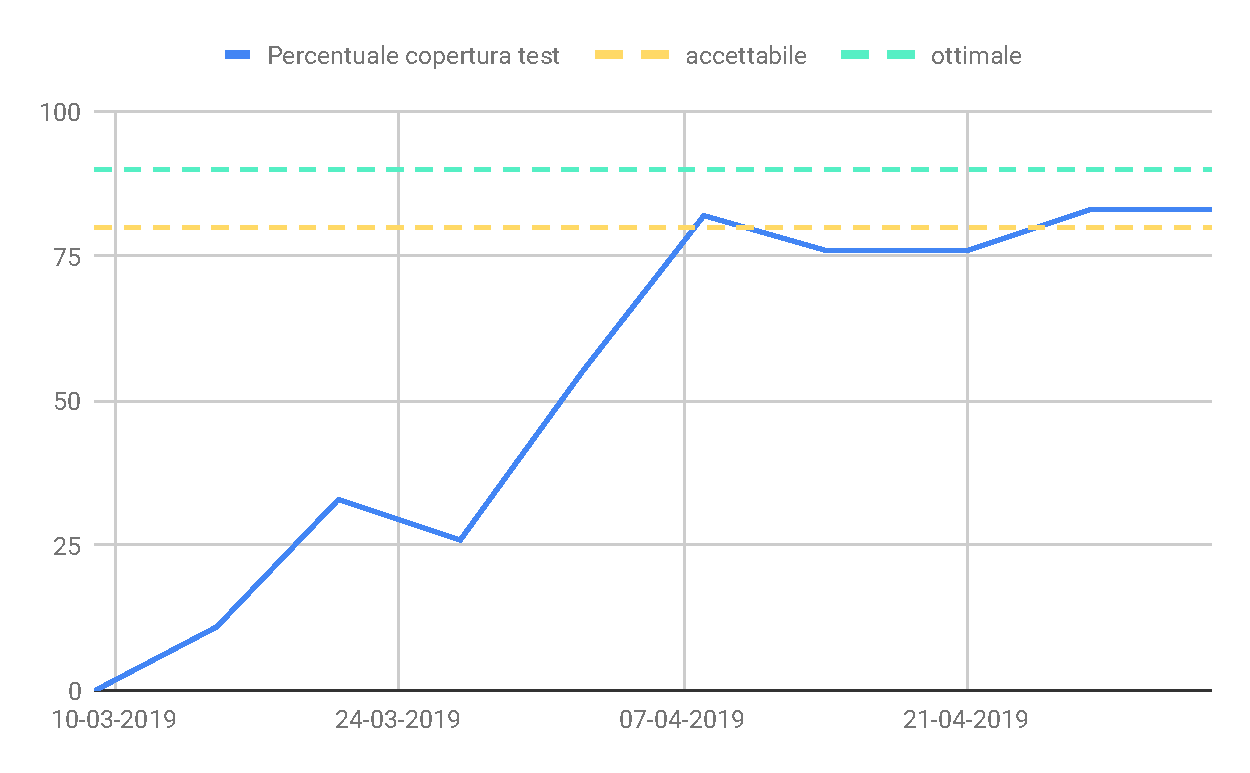
\includegraphics[width=145mm]{sez/App_Esito/Approvazione/graph/codeCoverage.pdf}
        \caption{Storico Code Coverage alla revisione di Approvazione}
    \end{figure}

\paragraph{MS008 - Superamento test}\mbox{}\\[0,3cm]
    \begin{table}[H]
        \centering
        \begin{tabular}{cccc}
        \rowcolor{greySWEight}
        \textcolor{white}{\textbf{Codice}} &
        \textcolor{white}{\textbf{Nome}} &
        \textcolor{white}{\textbf{Valore}} &
        \textcolor{white}{\textbf{Riscontro}}\\
        \textbf{MS008}& Test superati & 100\% & \textcolor{ForestGreen}{Ottimale} \\

        \end{tabular}
        \caption{Percentuale di test superati alla revisione di Approvazione}
    \end{table}

\paragraph{MS009 - Soddisfacimento requisiti obbligatori}\mbox{}\\[0,3cm]
    \begin{table}[H]
        \centering
        \begin{tabular}{cccc}
        \rowcolor{greySWEight}
        \textcolor{white}{\textbf{Codice}} &
        \textcolor{white}{\textbf{Requisiti obbligatori soddisfatti}} &
        \textcolor{white}{\textbf{Riscontro}}\\
        \textbf{MS009}& 100\% & \textcolor{ForestGreen}{Ottimale} \\

        \end{tabular}
        \caption{Requisit obbligatori soddisfatti alla revisione di Approvazione}
    \end{table}

\paragraph{MS010 - Media di build Travis settimanali}\mbox{}\\[0,3cm]
    

    \begin{table}[H]
        \centering
        \begin{tabular}{cccc}
        \rowcolor{greySWEight}
        \textcolor{white}{\textbf{Codice}} &
        \textcolor{white}{\textbf{Media}} &
        \textcolor{white}{\textbf{Riscontro}}\\
        \textbf{MS010}& 69.37 & \textcolor{ForestGreen}{Ottimale} \\
    
        \end{tabular}
        \caption{Media build settimanali alla revisione di Approvazione}
    \end{table}
    \begin{figure}[H]
        \centering
        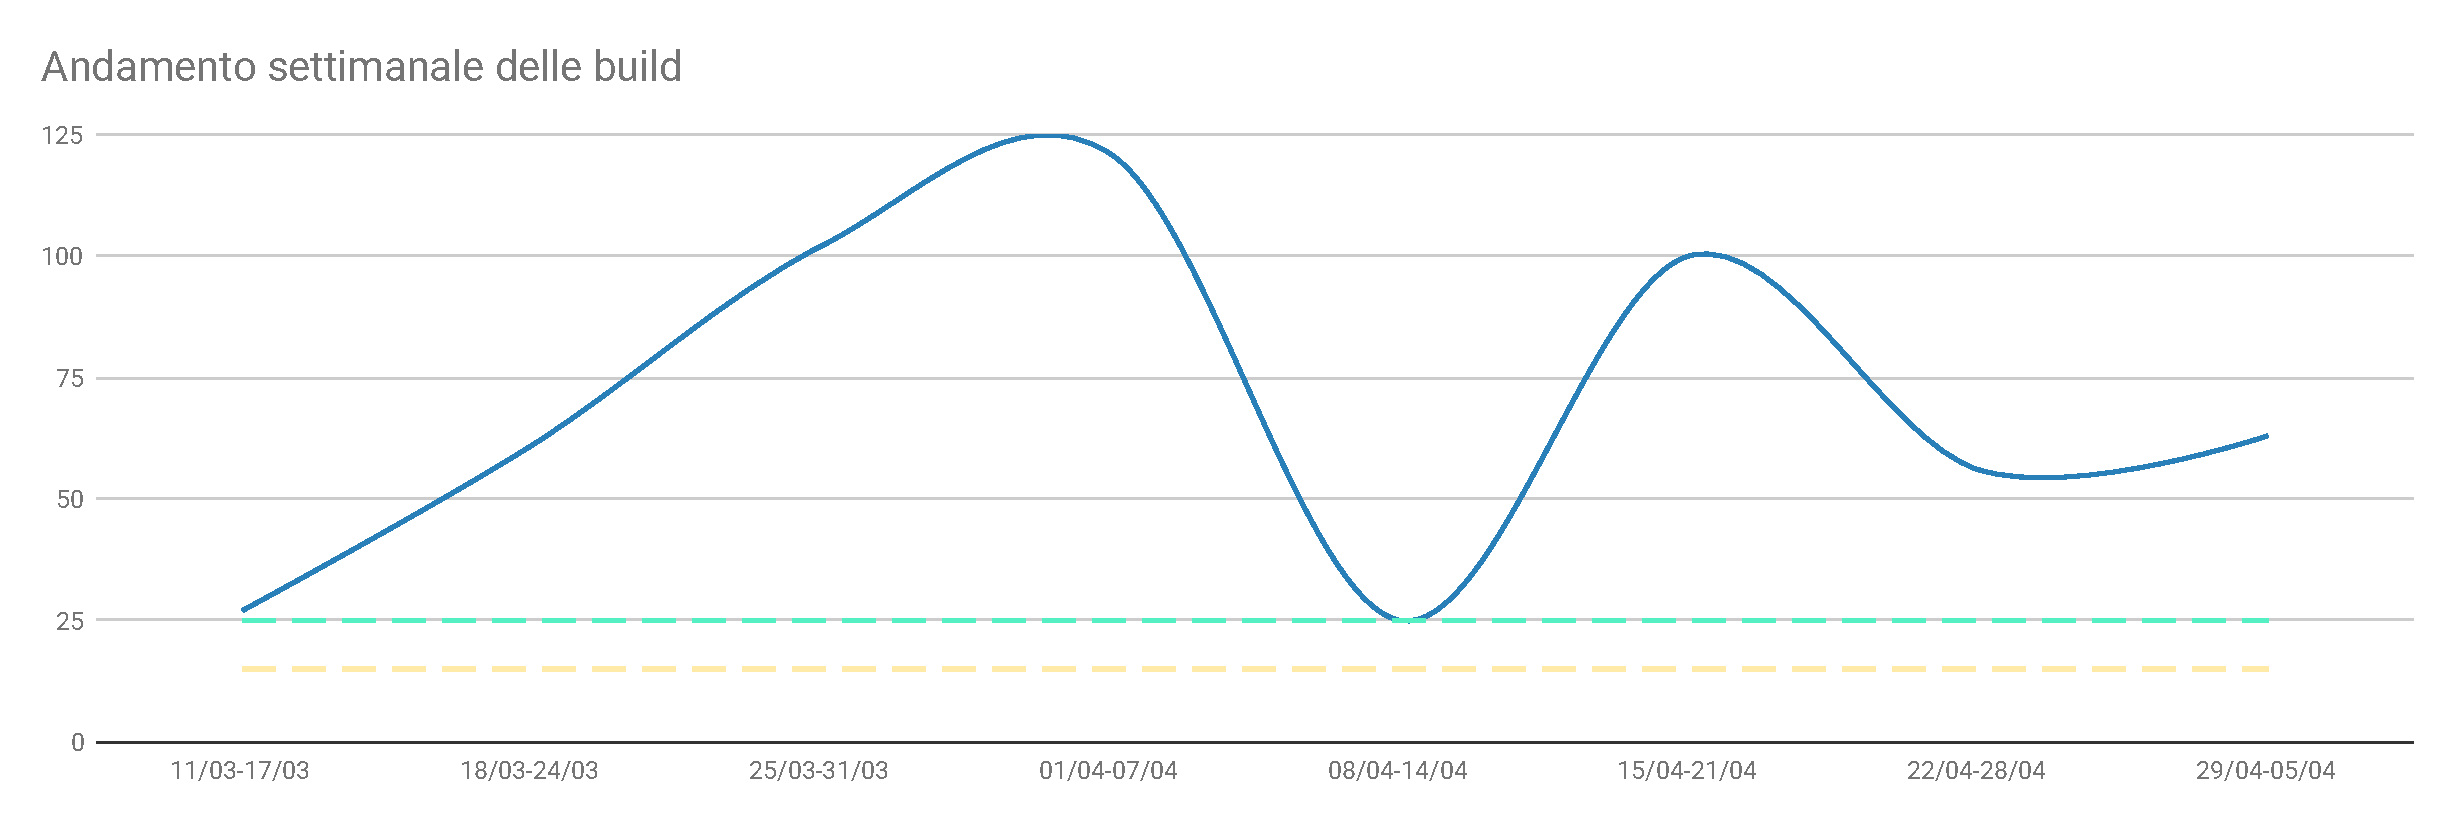
\includegraphics[width=165mm]{sez/App_Esito/Approvazione/graph/buildSettimanaliStorico.pdf}
        \caption{Build di Travis settimanali, dal 2019-03-11 al 2019-05-04}
    \end{figure}
    \begin{figure}[H]
        \centering
        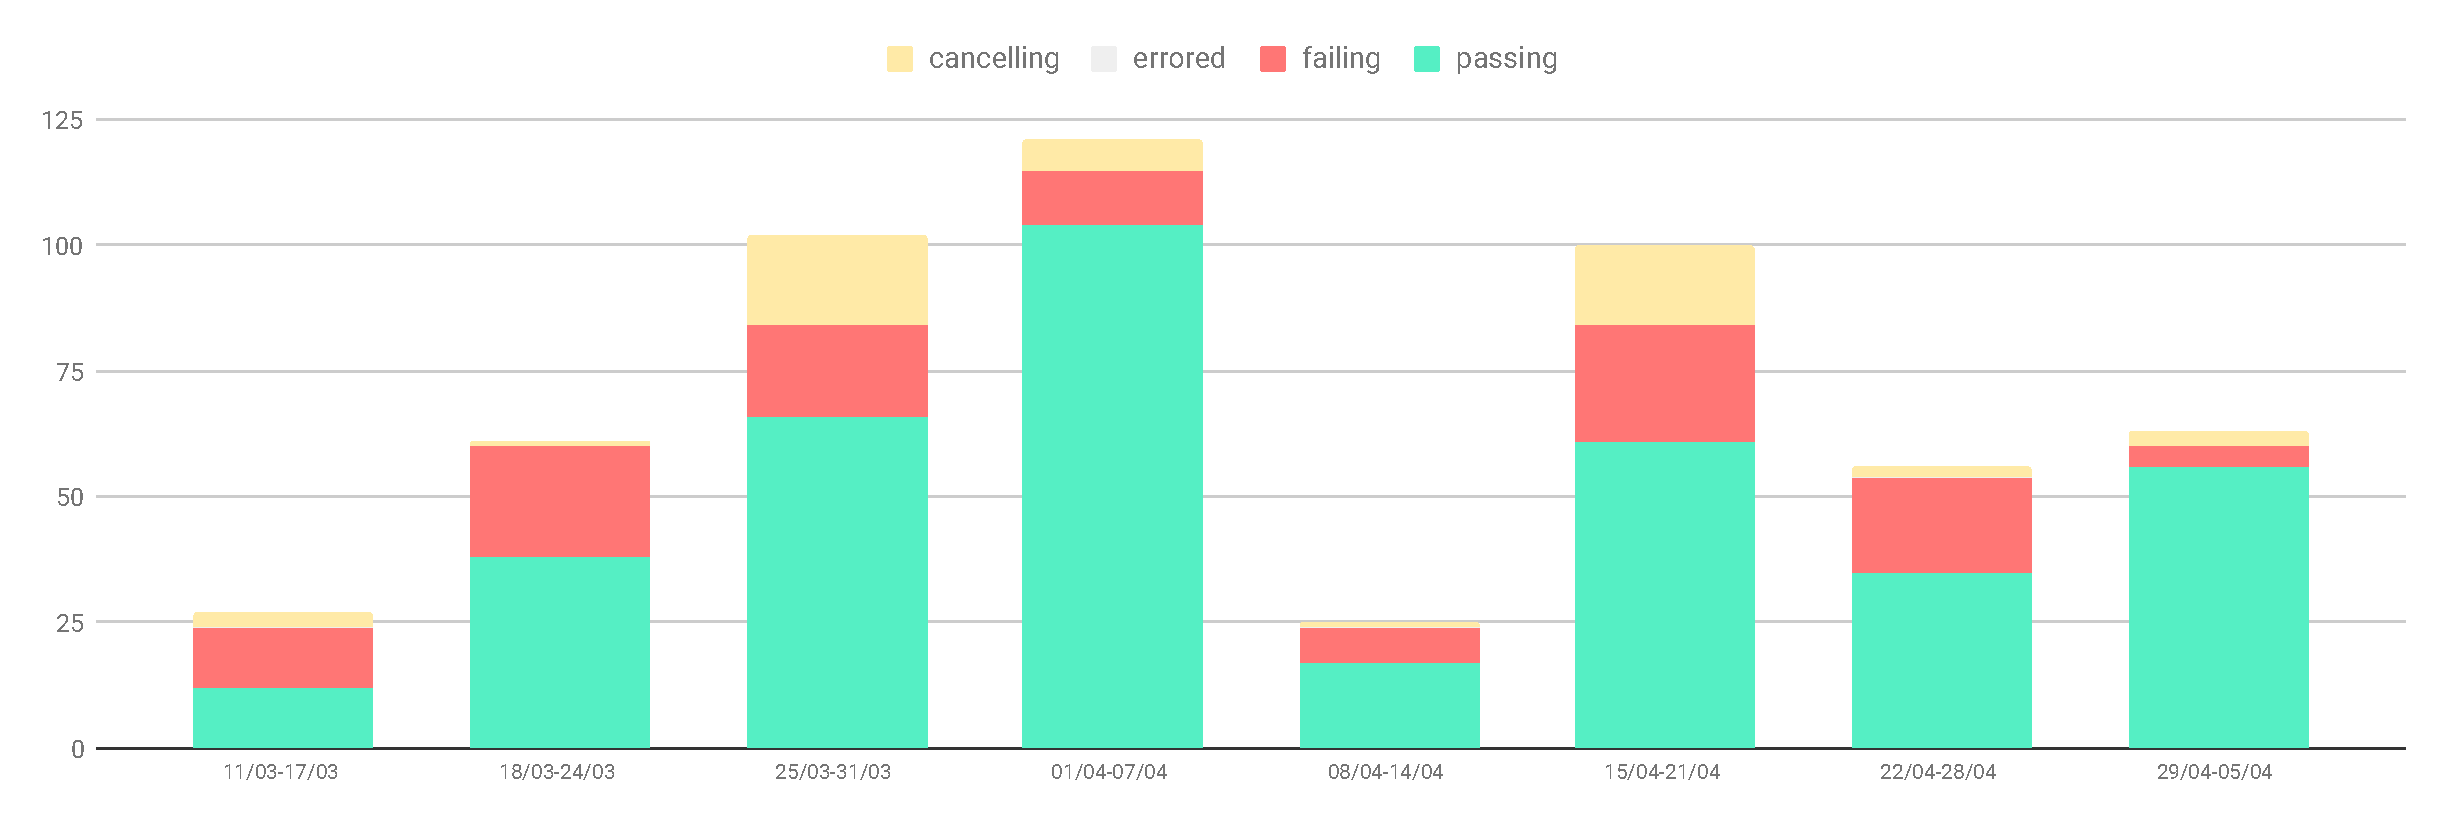
\includegraphics[width=165mm]{sez/App_Esito/Approvazione/graph/buildSettimanali.pdf}
        \caption{Build di Travis settimanali Istogramma, dal 2019-03-11 al 2019-05-04}
    \end{figure}

    \paragraph{MS011 - Percentuale build Travis superate }\mbox{}\\[0,3cm]
    \begin{table}[H]
        \centering
        \begin{tabular}{c c c c c}
        \rowcolor{greySWEight}
        \textcolor{white}{\textbf{Codice}} &
        \textcolor{white}{\textbf{Range accettabile}} &
        \textcolor{white}{\textbf{Range ottimale}} &
        \textcolor{white}{\textbf{build superate}} &
        \textcolor{white}{\textbf{Riscontro}}\\
        \textbf{MS011} & $[75\%,100\%]$ & $[85\%,100\%]$ & 71.40\% & \textcolor{YellowOrange}{Accettabile} \\
    
        \end{tabular}
        \caption{Build Travis superate alla revisione di Approvazione}
    \end{table}
    \begin{figure}[H]
        \centering
        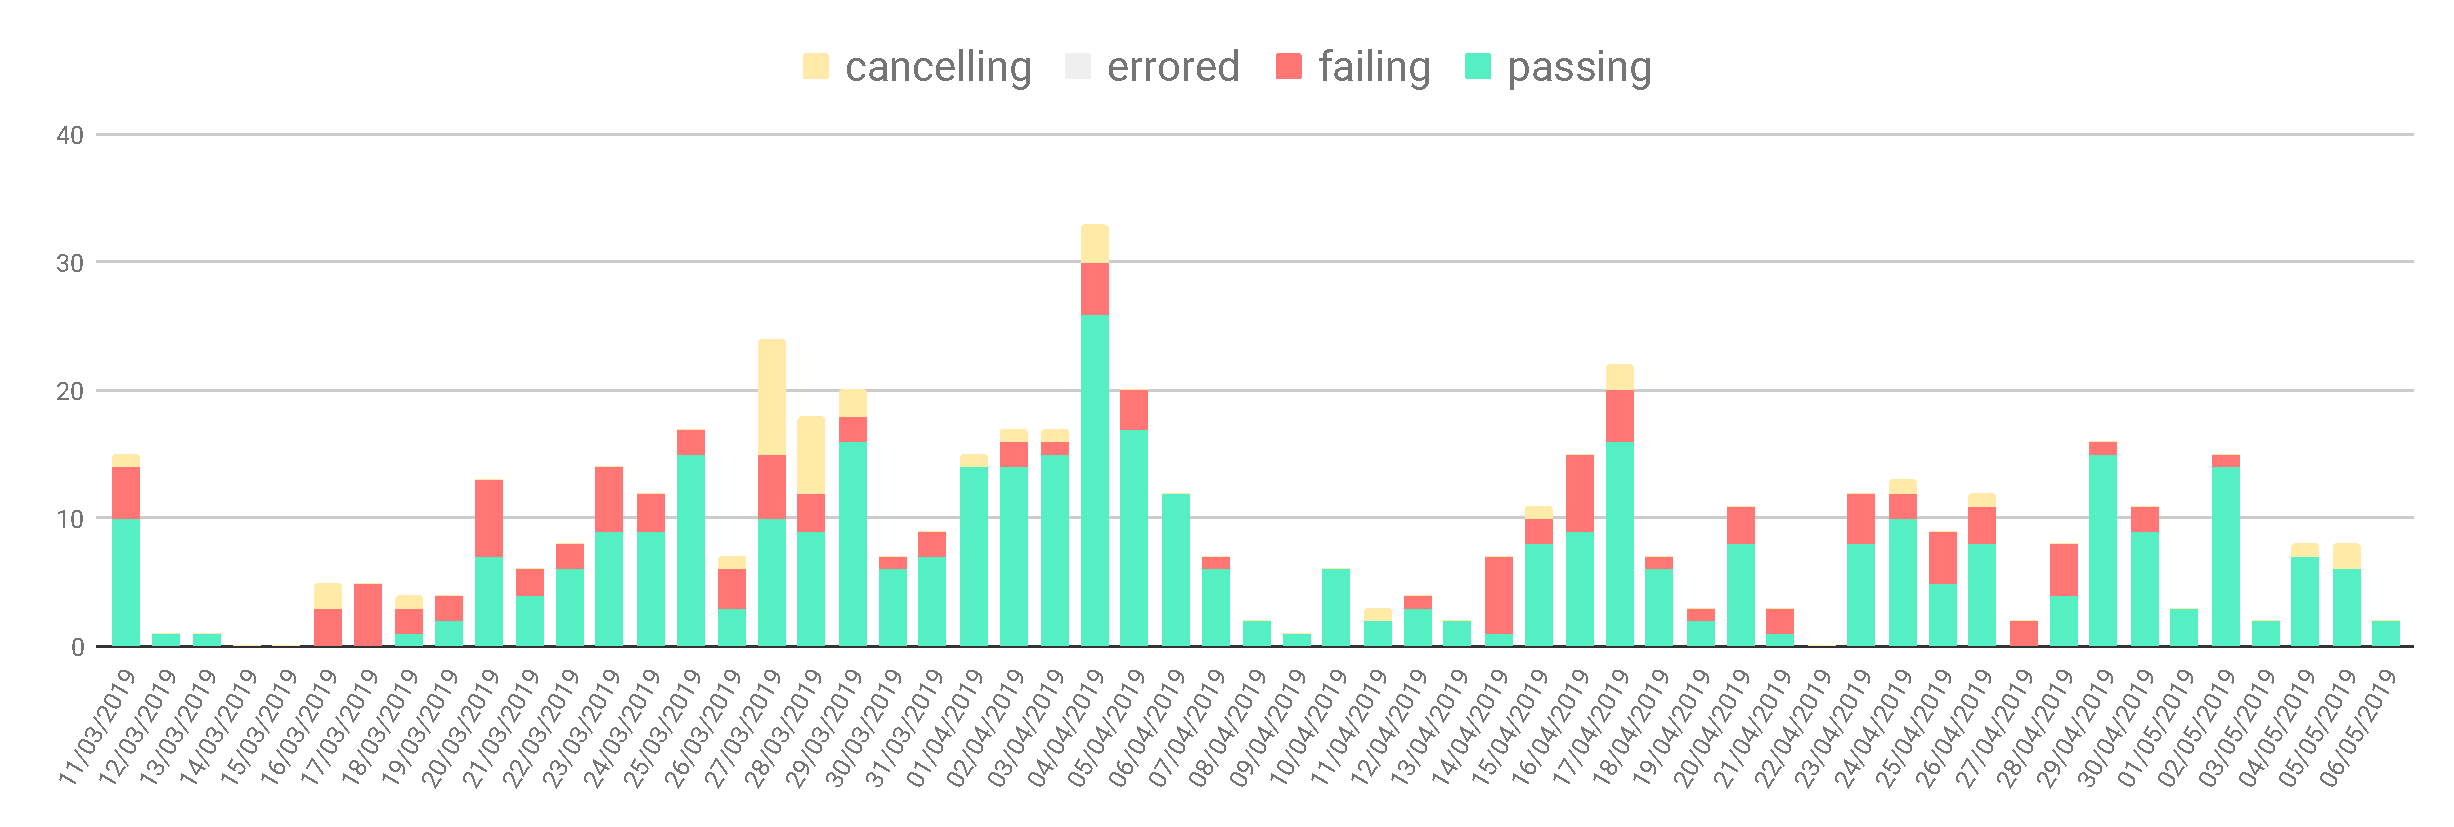
\includegraphics[width=165mm]{sez/App_Esito/Approvazione/graph/buildGiornaliere.pdf}
        \caption{Build di Travis giornaliere, dal 2019-03-11 al 2019-05-04}
    \end{figure}
    \begin{figure}[H]
        \centering
        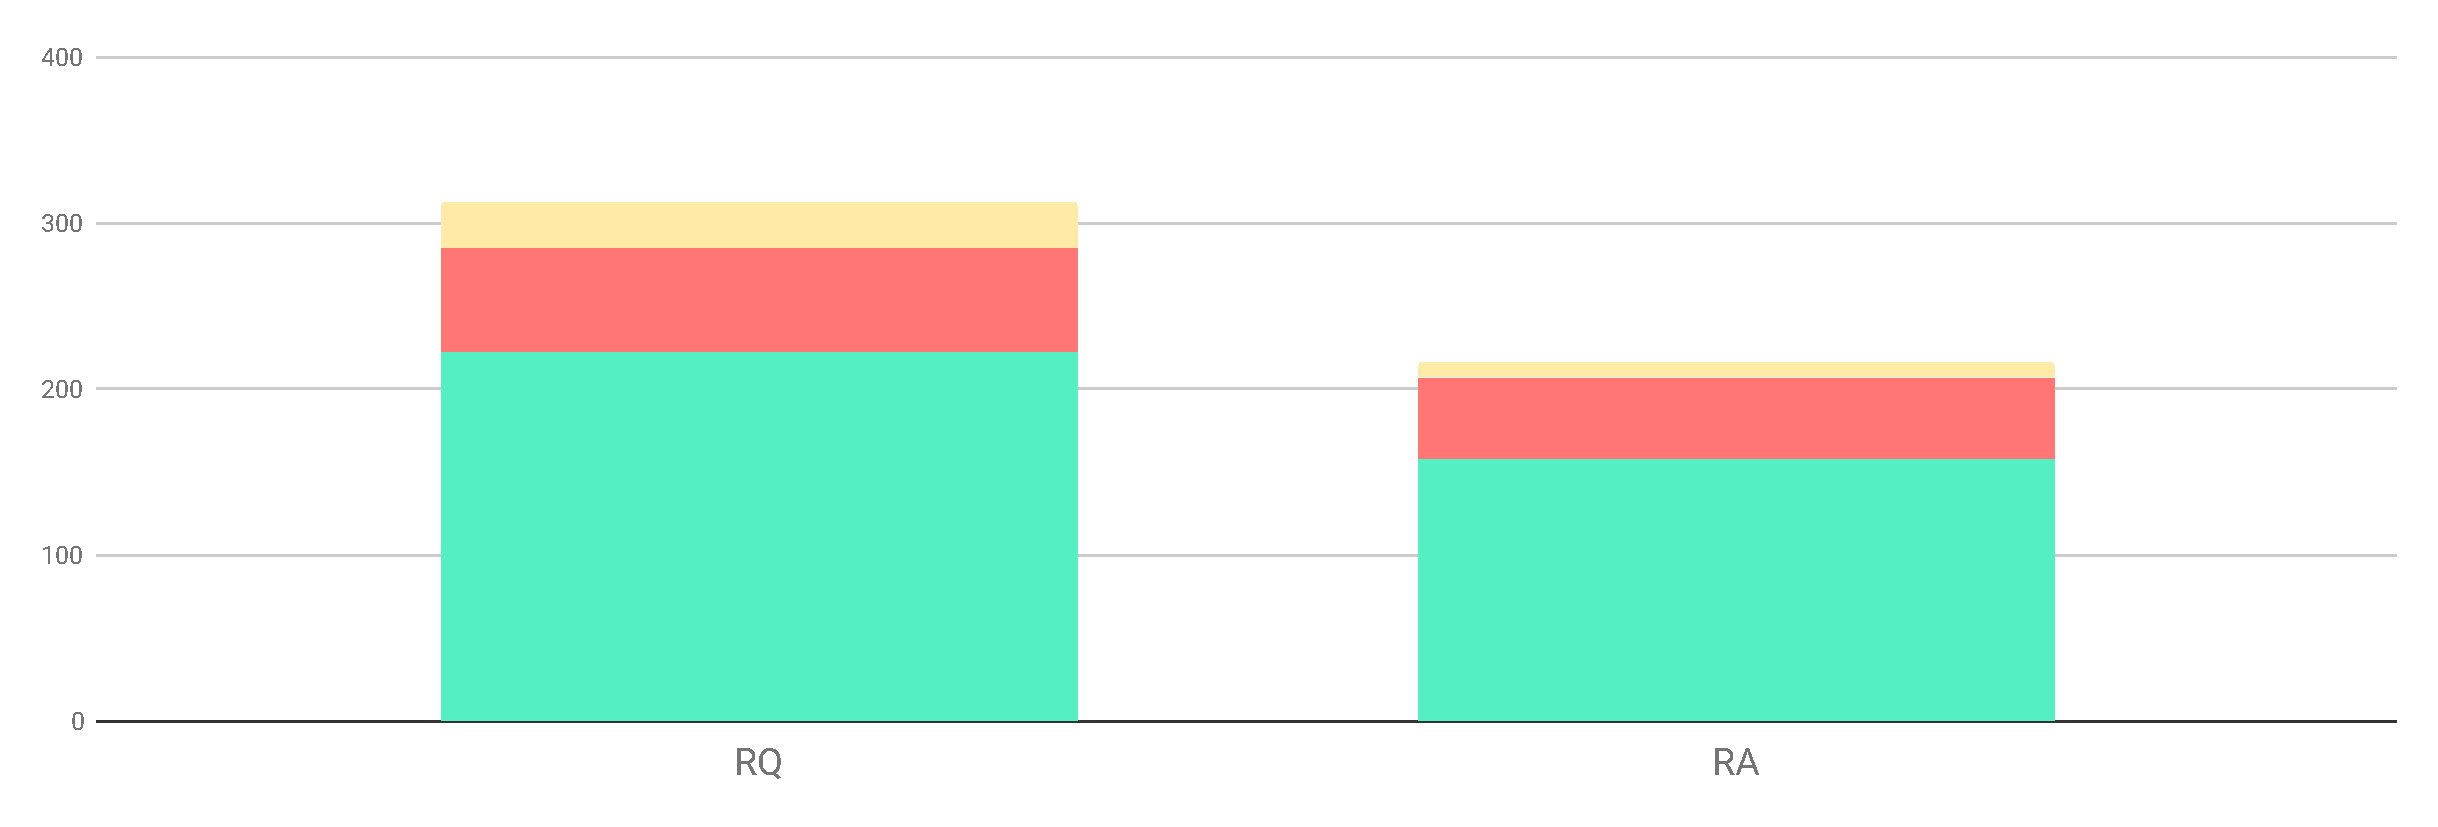
\includegraphics[width=165mm]{sez/App_Esito/Approvazione/graph/buildGiornaliereConfronto.pdf}
        \caption{Confronto build Travis RQ e RA}
    \end{figure}
    \begin{figure}[H]
        \centering
        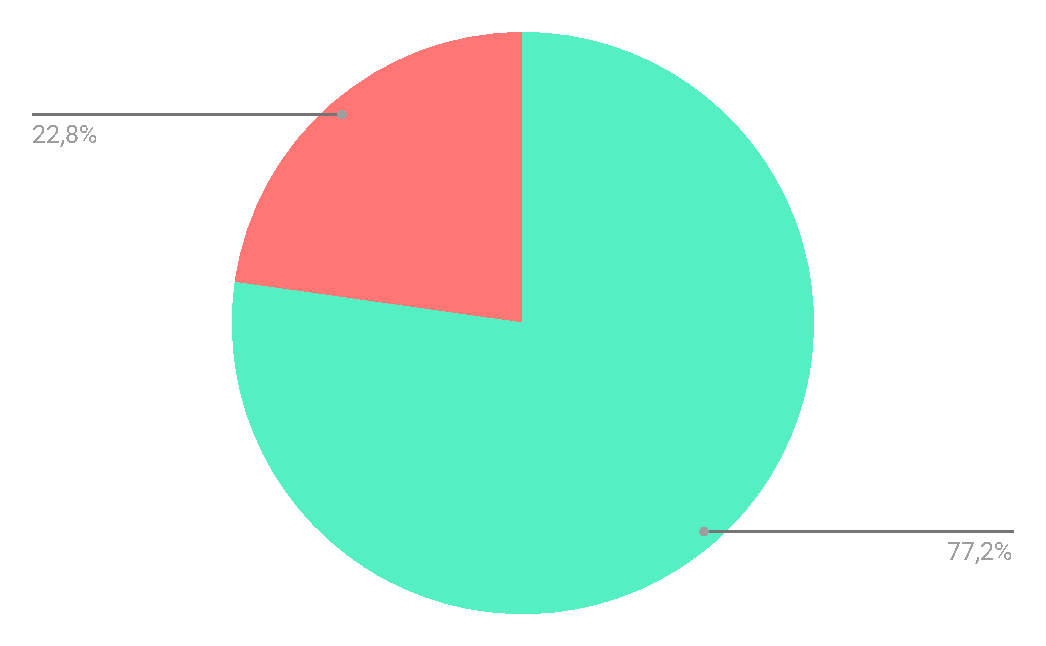
\includegraphics[width=100mm]{sez/App_Esito/Approvazione/graph/buildSuperateTorta.pdf}
        \caption{Build di Travis superate alla revisione di Approvazione}
    \end{figure}